\documentclass[12pt]{article}
\usepackage{amsmath}
\usepackage{amssymb}
\usepackage{graphicx}
\usepackage{hyperref}
\usepackage[latin1]{inputenc}
\usepackage{listings}
\usepackage{pgfplots}
\renewcommand{\labelitemi}{$\textendash$}
\renewcommand{\arraystretch}{1.4}

\title{ST3009: Week 9 Assignment}
\author{Conor McCauley - 17323203}
\date{March 30, 2020}

\begin{document}

\maketitle

\section*{Question 1}

\noindent (a) The following Python code runs the gradient descent algorithm on a given function for a number of different learning rate parameters. It also plots the results.

\begin{lstlisting}[language=Python]
    from random import uniform
    import matplotlib.pyplot as plt
    
    def gradient_descent(df, alpha, start_x, iterations):
    	theta = [None] * iterations
    	theta[0] = start_x
    	for i in range(1, iterations):
    		theta[i] = theta[i - 1] - (alpha * df(theta[i - 1]))
    	return theta
    
    f = lambda x: (x * x) - 1
    df = lambda x: 2 * x
    start_x = uniform(-1, 1)  # start at a random point
    iterations = 100  # number of iterations to run
    
    for alpha in [1.0, 0.1, 0.01]:
    	results = gradient_descent(df, alpha, start_x, iterations)
    	plt.plot(list(map(f, results)))
    	plt.show()
\end{lstlisting}

\noindent (b) The above code produces the following plots:

\begin{center}
    
    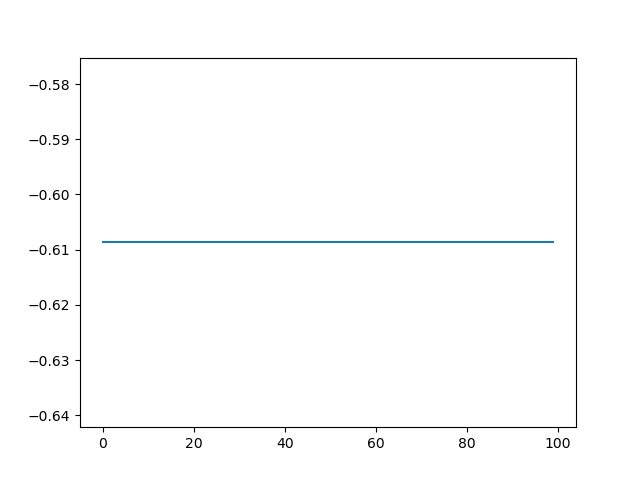
\includegraphics[scale=0.6]{q1_grad_plot_1.png}
    
    $\alpha = 1.0$
    
    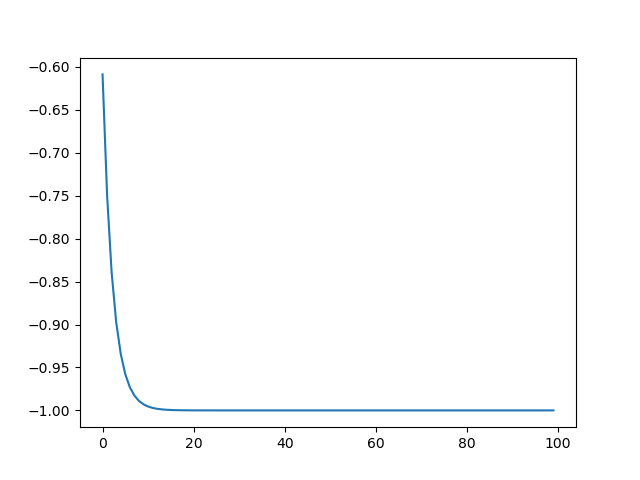
\includegraphics[scale=0.6]{q1_grad_plot_2.png}
    
    $\alpha = 0.1$
    
    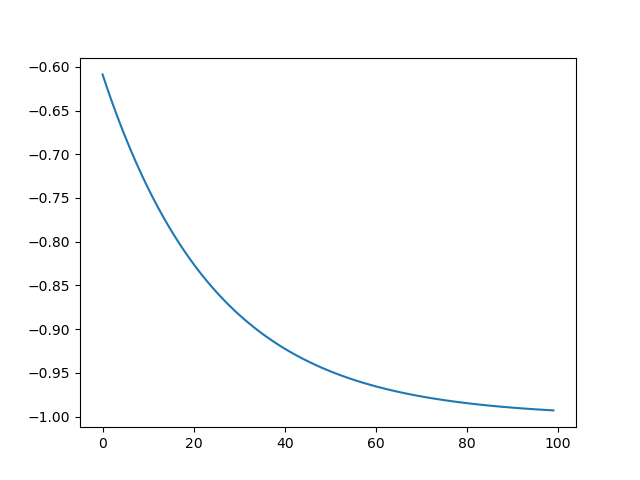
\includegraphics[scale=0.6]{q1_grad_plot_3.png}
    
    $\alpha = 0.01$
    
\end{center}

\indent It is clearly evident from the first plot that a learning rate of $\alpha = 1.0$ is much too large as there is no descent whatsoever - even after 100 iterations. The second plot, where $\alpha = 0.1$, quickly descends to the minimum in less than 20 iterations, while the final plot, where $\alpha = 0.01$, takes almost 100 iterations to reach the minimum: 5 times longer than the previous plot.

\indent It appears that a learning rate of $\alpha = 0.1$ is the optimal solution for the function $f(x) = x^2 - 1$ as it neither overshoots the minimum nor require a large number of iterations to converge on the minimum.

\noindent (c) The following Python code implements the {\it `random point'} algorithm and plots the result:

\begin{lstlisting}[language=Python]
    from random import uniform
    import matplotlib.pyplot as plt
    
    def random_point(f, max_step, start_x, iterations, max_tries):
    	results = [None] * iterations
    	results[0] = start_x
    	min_x = start_x
    	for i in range(1, iterations):
    		min_x = results[i - 1]
    		x = min_x
    		tries = 0
    		while f(x) >= f(min_x) and tries < max_tries:
    			x = min_x + uniform(-max_step, max_step)
    			tries += 1
    		# if we didn't run out of tries
    		if f(x) < f(min_x):
    			min_x = x
    		results[i] = min_x
    	return results
    
    f = lambda x: (x * x) - 1
    max_step = 0.1  # max absolute change in x after each iteration
    start_x = uniform(-1, 1)  # start at a random point
    iterations = 100  # number of iterations to run
    max_tries = 50  # max number of tries to descend each iteration
    
    results = random_point(f, max_step, start_x, iterations, max_tries)
    plt.plot(list(map(f, results)))
    plt.show()
\end{lstlisting}

\indent For each iteration the algorithm limits the {\it `vicinity'} of new $x$ values to those within the range $x \pm 0.1$ and limits the number of attempts to 50. The latter limitation prevents the occurrence of infinite loops. The code produces the following plot:

\begin{center}
    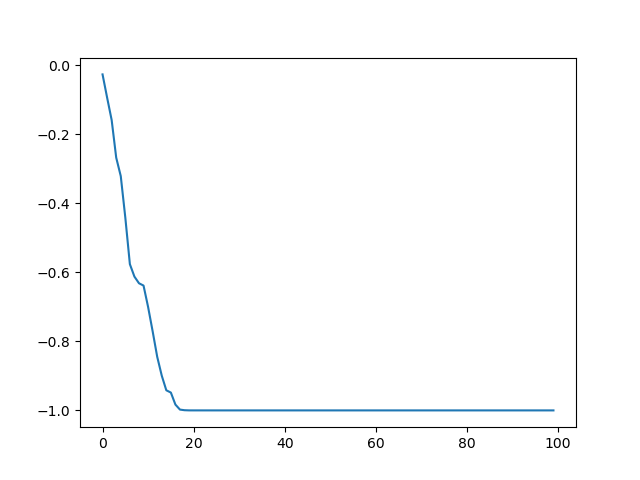
\includegraphics[scale=0.6]{q1_rand_plot.png}
\end{center}

\noindent (d) The randomised approach appears to converge on the minimum a little slower than the optimal gradient descent solution ($\alpha = 0.1$). However, the number of iterations needed to descend to the minimum is not an accurate representation of the amount of computation needed as it ignores the additional overhead of needing to randomly try many different nearby points during each iteration. It is clear that the gradient descent approach, with a somewhat optimal learning rate, is far more efficient that the randomised approach.

\section*{Question 2}

\noindent (a) We will label negative reviews as $-1$ and positive reviews as $+1$. In order to implement logistic regression we must define some kind of model which can be trained. We will refer to a review's feature vector as $x$ and to the overall parameter vector as $\theta$.

\indent We can define the model or hypothesis as $y = h_{\theta}(x)$ where $y = \pm 1$ (the classification) and $h_{\theta}(x)$ is the sign of the product of the transposed parameter vector and a review's feature vector: $sign(\theta^{T}x)$. Our training data can now be described as a series of inputs, $x^{(i)}$, and outputs, $y^{(i)}$, where $i$ refers to the $i^{th}$ datum in the training data.

\indent To train our model we must find values for the parameter vector $\theta$ that minimise the logistic regression cost function, $J(\theta)$, that was given in lectures (where $m$ is the amount of training data):

$$J(\theta) = \frac{1}{m} \sum_{i = 1}^m \log(1 + e^{-y^{(i)} \theta^T x^{(i)}})$$

\indent To minimise the cost function we simply use a gradient descent algorithm similar to the one given in question 1 (albeit a more complex version of the algorithm as we are working with an N-dimensional vector as opposed to a linear function).

\noindent (b) One of the key assumptions that this logistic regression classifier makes is that a review is either negative or positive. This assumed binary may not be entirely reflective of the content of a review since their content can be nuanced or portray mixed feelings.

\indent Another assumption that this classifier makes is that there is minimal collinearity between the entries in the feature vector. This is unlikely to be the case as, for example, entries like `bad' and `poor' are probably more likely to appear alongside each other than `bad' and `good'.

\noindent (c) To implement bootstrapping we can repeatedly select a sample (with replacement) of $N$ items of training data from our full set of training data and use this subset to train our model. This resampling method will allow us to randomly generate many different models from the same overall set of training data.

\indent We can test these models against a specified review (as stated in the question) and map the model to a $1$ if it classifies a review correctly or a $0$ if it classifies a review incorrectly. For example, six resampled models might give the following results: $\{ 1, 1, 0, 1, 0, 1 \}$ which would result in a mean correctness of $\frac{4}{6} = 0.\overline{6}$. Repeating this process many times will give us a distribution of means which we can use to estimate the confidence interval for the prediction accuracy of the classifier for the specified review.

\end{document}
